\documentclass[
	letterpaper, % Paper size, specify a4paper (A4) or letterpaper (US letter)
	10pt, % Default font size, specify 10pt, 11pt or 12pt
]{CSUniSchoolLabReport}

%----------------------------------------------------------------------------------------
%	REPORT INFORMATION
%----------------------------------------------------------------------------------------

\title{Analog to Digital Conversion and Sampling \\ Circuits \& Signals \\ EECE2150} % Report title

\author{Michael \textsc{Brodskiy}}

\date{February 23, 2023} % Date of the report

%----------------------------------------------------------------------------------------


\begin{document}

\maketitle % Insert the title, author and date using the information specified above

\begin{center}
	\begin{tabular}{l r}
		Date Performed: & February 23, 2023 \\ % Date the experiment was performed
        Partner: & Juan \textsc{Zapata} \\ % Partner names
		Instructor: & Professor \textsc{Sun} % Instructor/supervisor
	\end{tabular}
\end{center}

\setcounter{section}{-1}

\section{Introduction}

The purpose of this laboratory experimentation is to familiarize oneself with analog to digital converters, as well as using said converters for real-world sampling. The analog to digital converter (ADC) was used to generate various waveforms, as well as receive a real-world sound signal.

\section{Code Integration}

\lstinputlisting[
    caption=Code Used to Integrate ADC, % Caption above the listing
	label=lst:L1, % Label for referencing this listing
	language=octave, % Use python functions/syntax highlighting
	frame=single, % Frame around the code listing
	showstringspaces=false, % Don't put marks in string spaces
	numbers=left, % Line numbers on left
	numberstyle=\tiny, % Line numbers styling
    backgroundcolor=\color{black!5}, % Set background color
    keywordstyle=\color{magenta!80}, % Set keyword color
    commentstyle=\color{blue!80}, % Set comment color
    stringstyle=\color{green!80}, % Set string color
    breaklines=true
  ]{Figures/L8Code.m}

  \begin{figure}[h!]
    \centering
    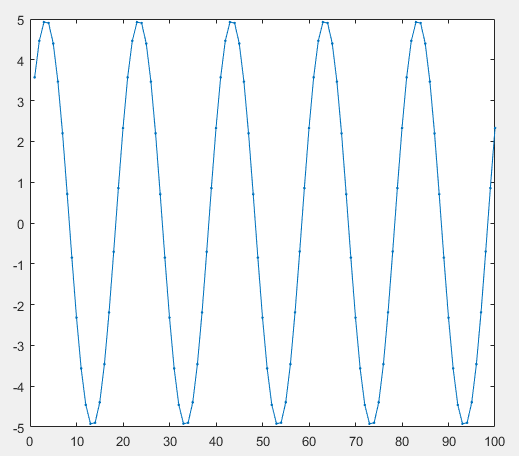
\includegraphics[width=.9\textwidth]{Figures/L8PL.png}
    \caption{A Generated Test Waveform}
    \label{fig:1}
  \end{figure}

  \begin{figure}[h!]
    \centering
    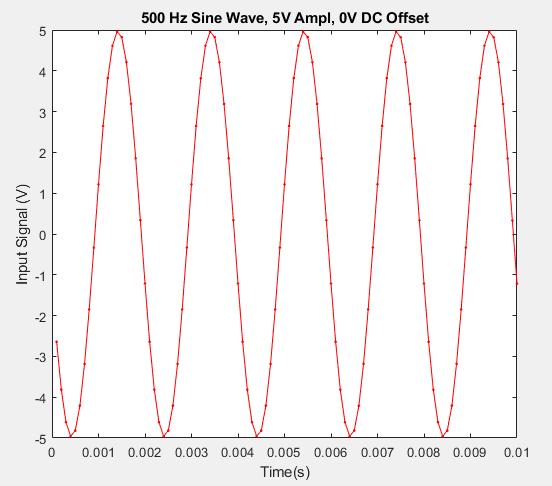
\includegraphics[width=.9\textwidth]{Figures/L8P2.png}
    \caption{Initial Waveform Configuration}
    \label{fig:2}
  \end{figure}

  \section{Part III\footnote{Parts I and II contained no questions, and, as such, were omitted}}

  \subsection{1}

  \subsubsection{i} \begin{figure}[h!]
    \centering
    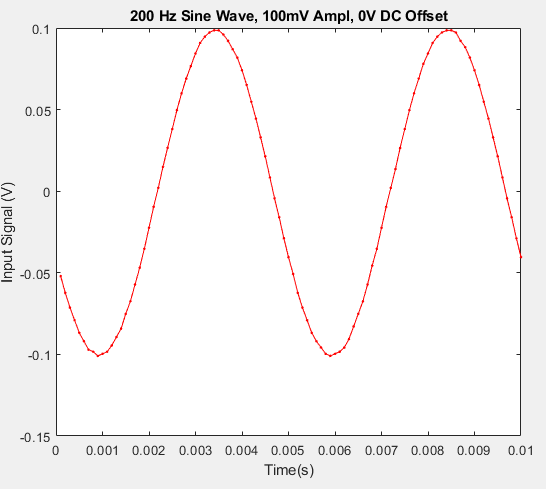
\includegraphics[width=.9\textwidth]{Figures/L8Config1.png}
    \caption{Waveform Generated in Configuration 1}
    \label{fig:3}
  \end{figure}

  \subsubsection{ii} The generated waveform, pictured above in Figure \ref{fig:3}, matches our expectations. It has approximately $.1[\si{\milli\volt}]$ of amplitude, and a period of $.005[\si{\second}]$, which is expected. Additionally, there is no vertical DC shift.

  \subsubsection{iii} There appear to be no problems with the waveform, other than that the graph does not appear to be entirely smooth.

  \subsection{2}

  \subsubsection{i} \begin{figure}[h!]
    \centering
    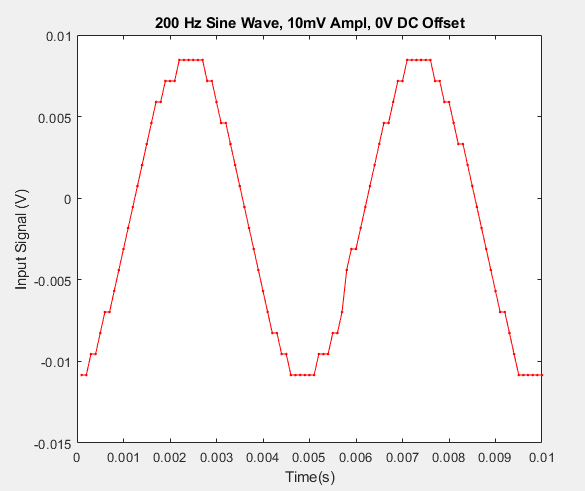
\includegraphics[width=.9\textwidth]{Figures/L8Config2.png}
    \caption{Waveform Generated in Configuration 2}
    \label{fig:4}
  \end{figure}

  \subsubsection{ii} The graph does not match our expectations perfectly; though the amplitude and period are correct, there is what appears to be a DC offset, as well as very low image quality.

  \subsubsection{iii} The problem is caused by the fact that the ADC can not draw changes in voltage that are that small, which makes the graph choppy and rounds down the voltage to the closest step.

  \subsubsection{iv} The problem can most likely be solved only by increasing the voltage.

  \subsection{Q1} A 14-bit register may hold:

  $$2^{14}=16384\text{ values}$$

  The step difference would be:

  $$\dfrac{20}{2^{14}}=1.22\cdot10^{-3}[\si{\volt}]$$

  This explains the above observations, as there are 8 distinct voltage levels in the interval $V=(.1,0)$. By calculating this, we obtain:

  $$\frac{.01}{8}=.00125$$

  This value is very close to the estimated step above, which explains why the plot can only plot certain values within this step range.

\section{Part IV}

\subsection{Q2} Because the noise being heard is within human range, it has to be somewhere from $20-20,000[\si{\hertz}]$. More specifically, it is most likely between $2,000-5,000[\si{\hertz}]$ because this range is most easily audible for humans.

\subsection{Q3} In order to best measure the amplitude of the signals, it is best to sample at least 10 times as much as the greatest frequency of the noise. This would explain why the 20k recording sounded similar to the original noise, but the 5k, 3k and 1k recordings are very different.

\subsection{Q4} This explains our results, as, because the noise is most likely in the range of $2,000-5,000[\si{\hertz}]$, 20k is the only sampling rate close enough to adequately record the noise.

\section{Conclusion}

Overall, this laboratory experiment introduced us to the concept of analog to digital converters (ADCs) through the use of MATLAB integration. This, together with the real-world examples involving various noises and frequencies, provided an adequate foundation for ADCs.

\end{document}
